\documentclass{llncs}
\usepackage[portuges]{babel}
\usepackage[utf8x]{inputenc}
\usepackage[T1]{fontenc}
\usepackage{graphicx}
\usepackage{fancyhdr}

\pagestyle{fancy}
\fancyhf{}
\rhead{João Calhau}
\rfoot{Page \thepage}

\begin{document}

\title{%
IoT Eye Tracking in Elderly Care}

\author{%
João Calhau}

\institute{%
  Universidade de Évora, Portugal\\
  \email{m36764@alunos.uevora.pt}\\
  \today
 }

\date{\today}

\maketitle{}

\begin{abstract}
A ideia de conectar objetos é discutida desde 1991, quando a Internet que conhecemos hoje começou a ganhar popularidade. Em 1999, Kevin Ashton do MIT propôs um termo, "Internet das Coisas". Essa ideia, esse termo, tem vindo a ganhar tração e ultimamente tem sido muito usado e falado nas redes sociais. Uns dos tópicos em que a Internet das coisas é mencionada é \textit{"Eye Tracking"} e \textit{"Elderly Care"}, e é precisamente destes tópicos que aqui venho falar hoje.
\end{abstract}


\section{Introdução}

Este \textit{Short Paper} enquadra-se no âmbito da disciplina de Computação Ubíqua, e serão abordados os temas \textit{Internet of Things}, \textit{Eye Tracking} e como estes dois se podem vir a enquadrar no dia-a-dia de uma pessoa Idosa.\\
\indent É objetivo deste \textit{Short paper} especificar o que é a \textit{Internet of Things}, ou Internet das coisas, em que consiste \textit{Eye Tracking}, como funciona e como se tem vindo a desenvolver e a evoluir nos dias correntes e juntar estes dois temas e tentar enquadra-los no dia-a-dia de uma pessoa idosa. "De que maneira pode ajudar?", "O que pode melhorar na sua vida?", "Que tarefas pode facilitar na sua vida?", são perguntas às quais tentarei responder até ao fim deste \textit{Short Paper}.\\
\indent Este \textit{Short Paper} está organizado em 3 partes. Na primeira parte será explicado o que é a Internet das Coisas, no que nos influencia e alguns exemplos de novidades do que tem vindo a trazer. Na segunda parte será explicado em que consiste \textit{Eye Tracking} e para que serve. Finalmente, na terceira parte falaremos um bocado das dificuldades que uma pessoa idosa tem todos os dias e como estes dois temas podem vir a ajudar a resolve-los.\\ 

\newpage

\lhead{IoT}

\section{\textit{Internet of Things}}
A Internet das coisas é uma revolução tecnológica que consiste em conectar objetos que usamos todos os dias a uma rede mundial, a Internet. A ideia da Internet das coisas é transformar o mundo digital e físico num só, através de dispositivos que comuniquem entre si. \cite{onl2} \\

\subsection{Aplicações}
Há vários tipos de aplicações possíveis para a Internet das coisas, entre elas podemos encontrar: 
\begin{itemize}
\item \textit{Connected Industry}, ou seja, coisas conectadas entre si na área da industria, como impressoras, guindastes e até minas inteiras. \cite{onl3}
\item \textit{Smart Cities}, cidades inteligentes que tem como objetivo criar condições de sustentabilidade, melhorar condições de vida da população através da análise de dados recolhidos das cidades.\cite{onl4}
\item \textit{Smart Energy}, redes elétricas inteligentes que utilizam a tecnologia da informação para fazer com que o sistema seja mais eficiente, tanto econômica como energeticamente. \cite{onl5}
\end{itemize}


\begin{figure}[!ht]
\centering
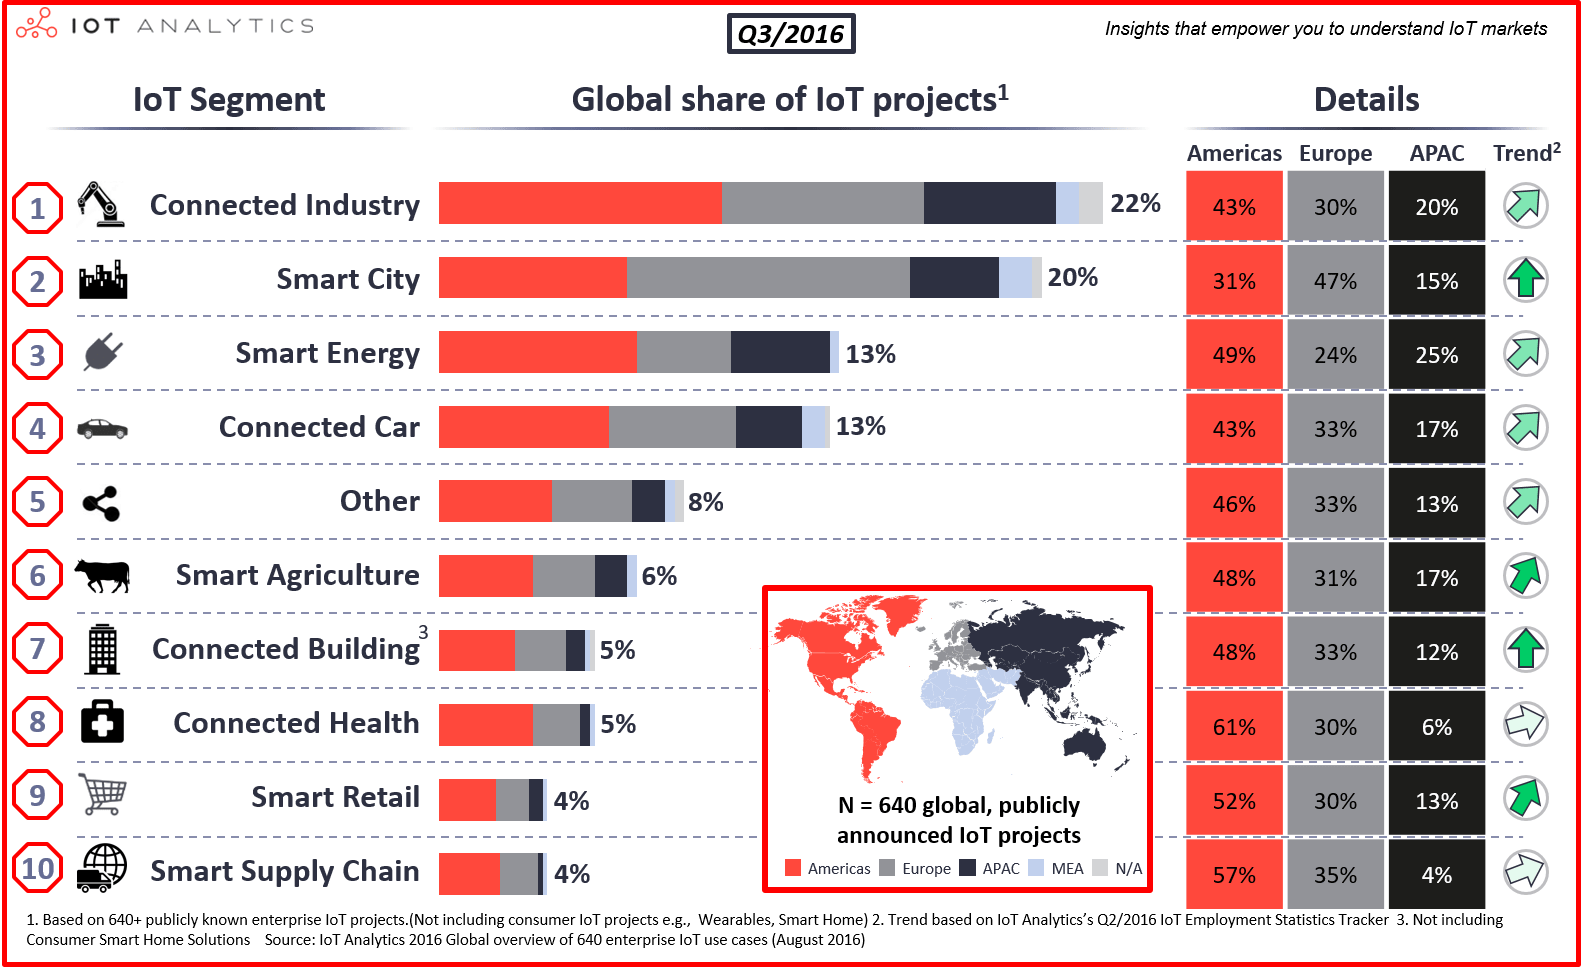
\includegraphics[width=120mm]{applications.png}
\caption{Top 10 áreas onde IoT está a ser aplicado \cite{onl3}}
\end{figure}

\newpage

\lhead{Eye Tracking}

\section{\textit{Eye Tracking}}
\textit{Eye Tracking} é um tipo de tecnologia sensorial que permite a um dispositivo saber exatamente onde é que os nossos olhos estão focados. Também consegue determinar a nossa presença, atenção, concentração, sonolência, entre outros. \cite{onl6}

\subsection{Aplicações}
Pensando em todas as vezes que podemos usar os nossos olhos durante um dia, ficamos rapidamente a perceber que \textit{Eye Tracking} tem muitas aplicações possíveis e como abrange tantas atividades no nosso dia-a-dia também percebemos que as áreas onde esta tecnologia se pode aplicar são as mais variadas. Com muito poucas exceções, qualquer coisa que tenha um componente visual pode ser "\textit{Tracked}". \textit{Eye Tracking} pode ser utilizado na área automóvel e médica a fim de nos tornar a vida mais segura, a área de entretenimento e web design já beneficiou significativamente estudando o comportamento visual do consumidor, todos os dias, à medida que \textit{Eye Tracking} é usado, é usado de maneiras novas e criativas e por isso a lista de aplicações possíveis cresce. \cite{onl7} 

\begin{figure}[!ht]
\centering
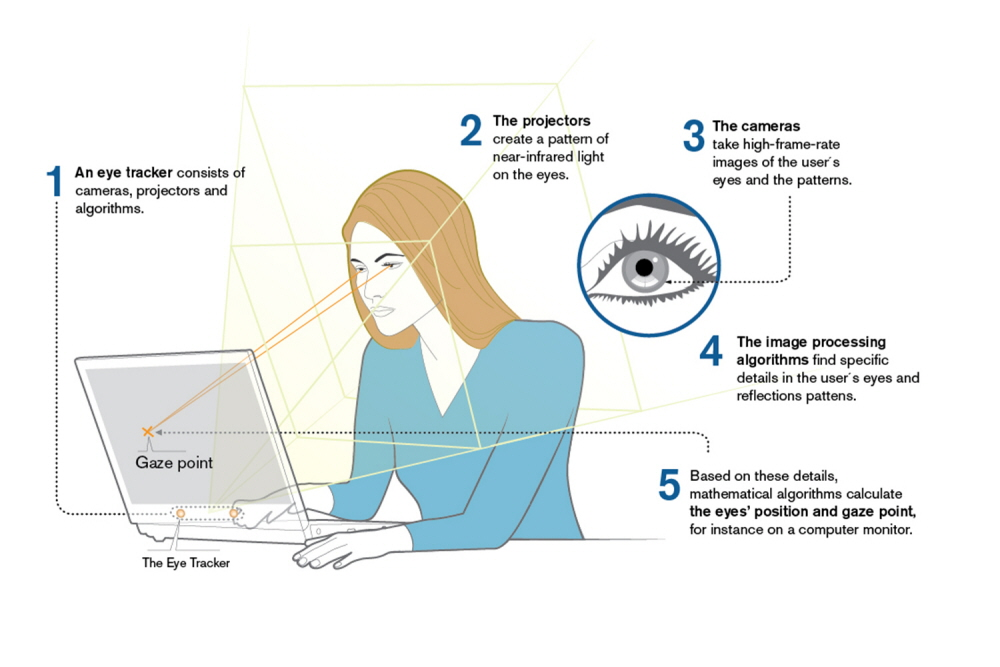
\includegraphics[width=120mm]{eyetracking.jpg}
\caption{No que consiste \textit{Eye Tracking} \cite{onl6}}
\end{figure}

\newpage

\lhead{Elderly Care}

\section{\textit{Elderly Care}}
Tendo falado já de \textit{IoT} e \textit{Eye Tracking} podemos agora falar destes dois tópicos focados numa área, a área dos cuidados ao idoso. \\
\indent \textit{Elderly Care}, ou cuidado ao idoso, é o cumprimento das necessidades especiais que são únicas a um idoso. O termo \textit{Elder Care}, engloba serviços como "viver com assistência" , "creches para adultos", "cuidados a longo prazo", entre outros. \cite{ar1} \\

\subsection{Aplicações}
\subsubsection{\textit{Interactive TVs}}
\textit{Interactive TVs}, ou televisões interativas, são uma das possíveis aplicações para a tecnologia de \textit{Eye Tracking}. As \textit{iTVs} são um aspeto particularmente interessante para uma pessoa idosa, pois permitiria o acesso a vários serviços a partir de casa. \cite{ar2} \\
\indent Os idosos constituem o maior grupo de consumidores de televisão e \textit{iTVs} providenciam aos idosos a oportunidade de estender o seu uso da televisão para atividades similares à Internet. Podem pesquisar informação, personalizar os seus hábitos de visualização, aceder a bases de dados, compras, apostas, e idealmente também interagir com outros utilizadores do mesmo sistema. \cite{ar2} \\

\begin{figure}[!ht]
\centering
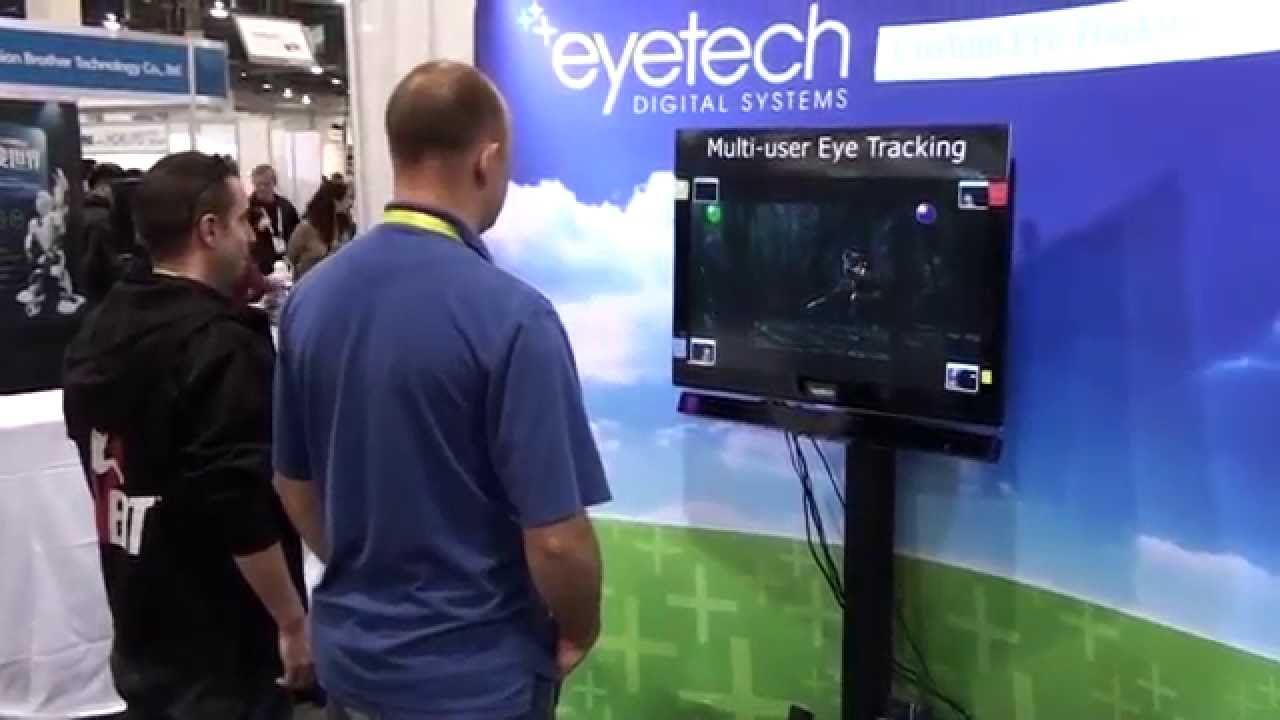
\includegraphics[width=120mm]{itv.jpg}
\caption{\textit{iTV} com seguimento de múltiplos olhos}
\end{figure}

\subsubsection{Condução}
Um idoso a conduzir nunca foi muito seguro, com a idade nota-se um abrandamento dos tempos de resposta, uma perda de claridade na visão e na audição, uma perda de força muscular e flexibilidade, uma certa sonolência por causa de certos tipos de medicamentos e uma reduzida habilidade de concentração. \cite{onl8} Mas \textit{Automotive Eye Tracking} tem a solução, deteta sonolência e avisa o condutor, deteta distração e dá avisos para encorajar ações evasivas, permite ainda um certo grau de personalização e identificação que permite o sistema reconhecer quem é o seu condutor e ajustar-se de acordo com as suas preferências. \cite{onl9}

\subsubsection{Medicina}
Com a tecnologia de \textit{Eye Tracking} até é possível detetar se uma pessoa idosa tem, ou não, Parkinson. o teste utiliza luz infravermelha para seguir o movimento dos olhos do paciente enquanto olham para um ecrã e seguem as instruções que lá aparecem. \cite{onl10} \\
\indent Hoje em dia, pessoas com a doença de Alzheimer são diagnosticadas depois de fazerem testes médicos detalhados e intensivos. Mas não há uma maneira rápida, barata e não invasiva capaz de identificar pessoas com essa doença. No entanto, há um método, ainda não acabado, capaz de testar essa doença de maneira não invasiva, a única coisa que o paciente tem de fazer é ver imagens num ecrã enquanto uma câmara segue os movimentos dos seus olhos.\cite{onl11}

\newpage

\lhead{Conclusão}

\section{Conclusão}
Neste \textit{Short Paper} abordei o assunto de \textit{Internet of Things}, \textit{Eye Tracking} e \textit{Elder Care} conclui, através da minha pesquisa, que embora ainda não haja muitas aplicações para \textit{Eye Tracking} inserido no tema de \textit{Elder care}, e as existentes ainda estarem a ser trabalhadas e aperfeiçoadas, esta nova tecnologia poderia melhorar significativamente o vida de uma pessoa idosa, tanto em termos de conforto como em utilidade ou como em diagnosticar doenças de maneira fácil, rápida e barata. \\
\indent Este trabalho foi muito importante para o meu conhecimento pois já conhecia o tema de Internet das Coisas, a área do \textit{Eye Tracking}, já tinha ouvido falar mas nunca me interessei muito por ela, mas vim a descobrir que até é bastante interessante. Desconhecia completamente que existiam métodos de diagnostico para as doenças de Alzheimer e Parkinson's através do seguimento dos olhos de uma pessoa, o que acabou por ser bastante interessante ficar a saber.

\newpage

\lhead{Referências}

\bibliographystyle{alpha}
\bibliography{bibliography}

\nocite{*}

\end{document}